% Created by tikzDevice version 0.6.2-92-0ad2792 on 2013-11-12 07:53:00
% !TEX encoding = UTF-8 Unicode
\documentclass[12pt, mainfont = Minion,     mainscale = 1.0, sansfont = Myriad,     sansscale = MatchLowercase, monofont = Consolas,   monoscale = MatchLowercase, mathfont = MinionMath, mathscale = 1.0]{mtikzfig}
\begin{document}

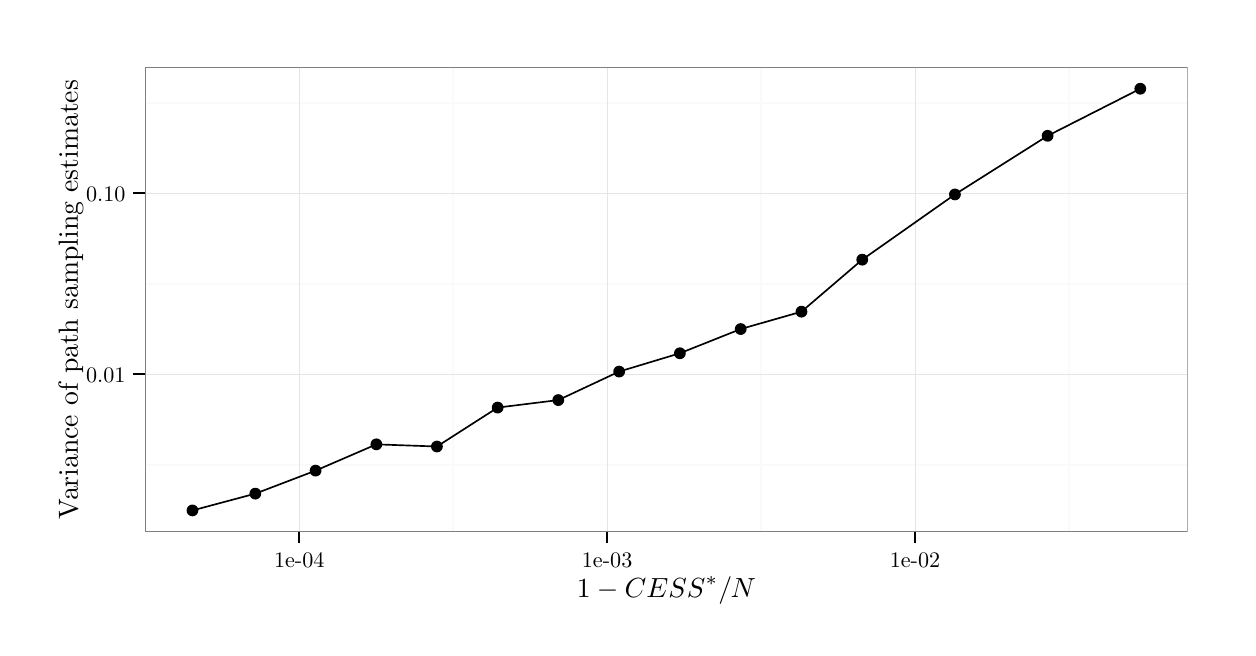
\begin{tikzpicture}[x=1pt,y=1pt]
\definecolor[named]{fillColor}{rgb}{1.00,1.00,1.00}
\path[use as bounding box,fill=fillColor,fill opacity=0.00] (0,0) rectangle (433.62,216.81);
\begin{scope}
\path[clip] (  0.00,  0.00) rectangle (433.62,216.81);
\definecolor[named]{drawColor}{rgb}{1.00,1.00,1.00}
\definecolor[named]{fillColor}{rgb}{1.00,1.00,1.00}

\path[draw=drawColor,line width= 0.6pt,line join=round,line cap=round,fill=fillColor] (  0.00,  0.00) rectangle (433.62,216.81);
\end{scope}
\begin{scope}
\path[clip] ( 42.43, 34.74) rectangle (419.17,202.36);
\definecolor[named]{fillColor}{rgb}{1.00,1.00,1.00}

\path[fill=fillColor] ( 42.43, 34.74) rectangle (419.17,202.36);
\definecolor[named]{drawColor}{rgb}{0.98,0.98,0.98}

\path[draw=drawColor,line width= 0.6pt,line join=round] ( 42.43, 58.85) --
	(419.17, 58.85);

\path[draw=drawColor,line width= 0.6pt,line join=round] ( 42.43,124.27) --
	(419.17,124.27);

\path[draw=drawColor,line width= 0.6pt,line join=round] ( 42.43,189.68) --
	(419.17,189.68);

\path[draw=drawColor,line width= 0.6pt,line join=round] ( 42.51, 34.74) --
	( 42.51,202.36);

\path[draw=drawColor,line width= 0.6pt,line join=round] (153.76, 34.74) --
	(153.76,202.36);

\path[draw=drawColor,line width= 0.6pt,line join=round] (265.02, 34.74) --
	(265.02,202.36);

\path[draw=drawColor,line width= 0.6pt,line join=round] (376.27, 34.74) --
	(376.27,202.36);
\definecolor[named]{drawColor}{rgb}{0.90,0.90,0.90}

\path[draw=drawColor,line width= 0.2pt,line join=round] ( 42.43, 91.56) --
	(419.17, 91.56);

\path[draw=drawColor,line width= 0.2pt,line join=round] ( 42.43,156.98) --
	(419.17,156.98);

\path[draw=drawColor,line width= 0.2pt,line join=round] ( 98.14, 34.74) --
	( 98.14,202.36);

\path[draw=drawColor,line width= 0.2pt,line join=round] (209.39, 34.74) --
	(209.39,202.36);

\path[draw=drawColor,line width= 0.2pt,line join=round] (320.65, 34.74) --
	(320.65,202.36);
\definecolor[named]{fillColor}{rgb}{0.00,0.00,0.00}

\path[fill=fillColor] ( 59.55, 42.36) circle (  2.13);

\path[fill=fillColor] ( 82.26, 48.43) circle (  2.13);

\path[fill=fillColor] (104.04, 56.75) circle (  2.13);

\path[fill=fillColor] (126.00, 66.24) circle (  2.13);

\path[fill=fillColor] (147.88, 65.46) circle (  2.13);

\path[fill=fillColor] (169.83, 79.53) circle (  2.13);

\path[fill=fillColor] (191.74, 82.24) circle (  2.13);

\path[fill=fillColor] (213.73, 92.54) circle (  2.13);

\path[fill=fillColor] (235.68, 99.16) circle (  2.13);

\path[fill=fillColor] (257.65,107.91) circle (  2.13);

\path[fill=fillColor] (279.61,114.18) circle (  2.13);

\path[fill=fillColor] (301.57,132.98) circle (  2.13);

\path[fill=fillColor] (335.06,156.55) circle (  2.13);

\path[fill=fillColor] (368.55,177.73) circle (  2.13);

\path[fill=fillColor] (402.04,194.74) circle (  2.13);
\definecolor[named]{drawColor}{rgb}{0.00,0.00,0.00}

\path[draw=drawColor,line width= 0.6pt,line join=round] ( 59.55, 42.36) --
	( 82.26, 48.43) --
	(104.04, 56.75) --
	(126.00, 66.24) --
	(147.88, 65.46) --
	(169.83, 79.53) --
	(191.74, 82.24) --
	(213.73, 92.54) --
	(235.68, 99.16) --
	(257.65,107.91) --
	(279.61,114.18) --
	(301.57,132.98) --
	(335.06,156.55) --
	(368.55,177.73) --
	(402.04,194.74);
\definecolor[named]{drawColor}{rgb}{0.50,0.50,0.50}

\path[draw=drawColor,line width= 0.6pt,line join=round,line cap=round] ( 42.43, 34.74) rectangle (419.17,202.36);
\end{scope}
\begin{scope}
\path[clip] (  0.00,  0.00) rectangle (433.62,216.81);
\definecolor[named]{drawColor}{rgb}{0.00,0.00,0.00}

\node[text=drawColor,anchor=base east,inner sep=0pt, outer sep=0pt, scale=  0.80] at ( 35.32, 88.63) {0.01};

\node[text=drawColor,anchor=base east,inner sep=0pt, outer sep=0pt, scale=  0.80] at ( 35.32,154.05) {0.10};
\end{scope}
\begin{scope}
\path[clip] (  0.00,  0.00) rectangle (433.62,216.81);
\definecolor[named]{drawColor}{rgb}{0.00,0.00,0.00}

\path[draw=drawColor,line width= 0.6pt,line join=round] ( 38.16, 91.56) --
	( 42.43, 91.56);

\path[draw=drawColor,line width= 0.6pt,line join=round] ( 38.16,156.98) --
	( 42.43,156.98);
\end{scope}
\begin{scope}
\path[clip] (  0.00,  0.00) rectangle (433.62,216.81);
\definecolor[named]{drawColor}{rgb}{0.00,0.00,0.00}

\path[draw=drawColor,line width= 0.6pt,line join=round] ( 98.14, 30.47) --
	( 98.14, 34.74);

\path[draw=drawColor,line width= 0.6pt,line join=round] (209.39, 30.47) --
	(209.39, 34.74);

\path[draw=drawColor,line width= 0.6pt,line join=round] (320.65, 30.47) --
	(320.65, 34.74);
\end{scope}
\begin{scope}
\path[clip] (  0.00,  0.00) rectangle (433.62,216.81);
\definecolor[named]{drawColor}{rgb}{0.00,0.00,0.00}

\node[text=drawColor,anchor=base,inner sep=0pt, outer sep=0pt, scale=  0.80] at ( 98.14, 21.77) {1e-04};

\node[text=drawColor,anchor=base,inner sep=0pt, outer sep=0pt, scale=  0.80] at (209.39, 21.77) {1e-03};

\node[text=drawColor,anchor=base,inner sep=0pt, outer sep=0pt, scale=  0.80] at (320.65, 21.77) {1e-02};
\end{scope}
\begin{scope}
\path[clip] (  0.00,  0.00) rectangle (433.62,216.81);
\definecolor[named]{drawColor}{rgb}{0.00,0.00,0.00}

\node[text=drawColor,anchor=base,inner sep=0pt, outer sep=0pt, scale=  1.00] at (230.80, 10.84) {$1 - \text{CESS}^*/N$};
\end{scope}
\begin{scope}
\path[clip] (  0.00,  0.00) rectangle (433.62,216.81);
\definecolor[named]{drawColor}{rgb}{0.00,0.00,0.00}

\node[text=drawColor,rotate= 90.00,anchor=base,inner sep=0pt, outer sep=0pt, scale=  1.00] at ( 18.16,118.55) {Variance of path sampling estimates};
\end{scope}
\end{tikzpicture}

\end{document}
